To establish this, observe that we can construct a consistent estimator for the model indicator $I$ by checking
for the equality of different outcomes.
Specifically, the estimator identifies outcomes with equal frequency in the data and returns the indicator for
the model that supports this equality.

To see how this idea works in practice, we carried out a synthetic experiment with the following setup.
We considered binary attributes and generated each feature independently with equal probability for 0 and 1.
The class label was defined as a deterministic function of a fixed subset of 3 out of 12 total attributes, as
shown in Table~\ref{tab:functions}.
The same relevant features and labeling function were used across all trials.

For each experiment, we generated a training set of size 20 and a test set of size 60.
A larger test set was used to reduce variability in performance estimates, taking advantage of the synthetic
nature of the data.
To assess robustness to irrelevant features, we progressively removed one attribute at a time from the full set
of 12, starting with irrelevant ones and stopping just before removing any of the three relevant features.

At each step, we trained and tested two versions of the central distribution: one assuming a deterministic label
function (CD-Det) and one allowing for a conditional (non-deterministic) label distribution (CD-Prob).
As a baseline, we also trained a decision tree classifier (DTree).
All methods were trained on the same training data and evaluated on the same test data.
Each configuration was repeated for 75 independent trials, and we reported the average accuracy (correct
predictions divided by total test instances) over these trials.

\begin{table}[htbp]
    \centering
    \caption{Mappings of 3-bit inputs under functions $f_1$ and $f_2$}
    \begin{tabular}{ccc}
        \toprule
        Input (bits) & $f_1$(Input) & $f_2$(Input) \\
        \midrule
        000          & a            & A            \\
        001          & b            & B            \\
        010          & c            & A            \\
        011          & d            & C            \\
        100          & e            & D            \\
        101          & f            & D            \\
        110          & g            & D            \\
        111          & h            & E            \\
        \bottomrule
    \end{tabular}\label{tab:functions}
\end{table}

\begin{figure}[htbp]
    \centering
    \caption{Accuracy vs. Number of Attributes (Function $f_1$, 20 train samples)}
    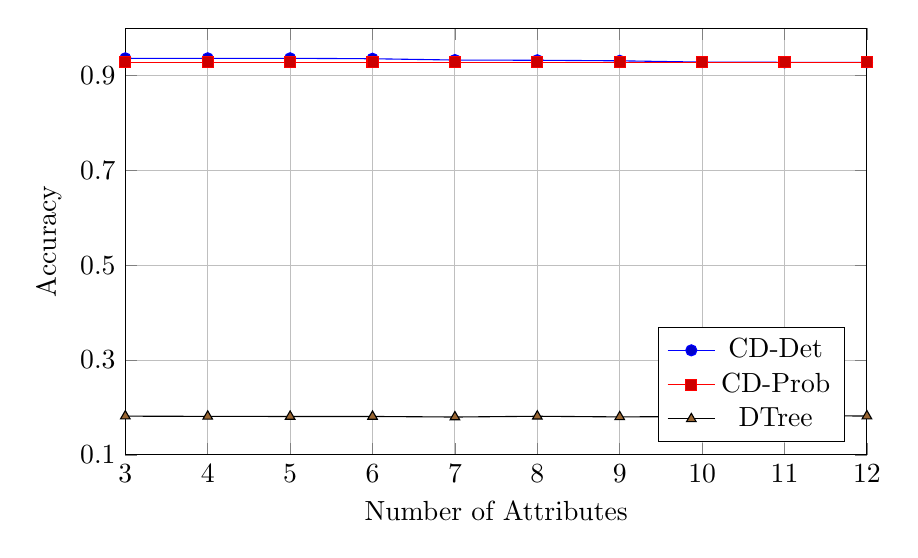
\begin{tikzpicture}
        \begin{axis}[
            width=11cm,
            height=7cm,
            xlabel={Number of Attributes},
            ylabel={Accuracy},
            xmin=3, xmax=12,
            ymin=0.1, ymax=1.0,
            xtick={3,4,5,6,7,8,9,10,11,12},
            ytick={0.1,0.3,0.5,0.7,0.9},
            legend pos=south east,
            grid=major,
            mark options={solid}
        ]

            \addplot+[mark=*, blue] coordinates {
                (3, 0.936541) (4, 0.936541) (5, 0.936541) (6, 0.935624) (7, 0.932875) (8, 0.932417) (9, 0.931271) (10, 0.928522) (11, 0.928064) (12, 0.928064)
            };
            \addlegendentry{CD-Det}

            \addplot+[mark=square*, red] coordinates {
                (3, 0.928064) (4, 0.928064) (5, 0.928064) (6, 0.928064) (7, 0.928064) (8, 0.928064) (9, 0.928064) (10, 0.928064) (11, 0.928064) (12, 0.928064)
            };
            \addlegendentry{CD-Prob}

            \addplot+[mark=triangle*, black] coordinates {
                (3, 0.181672) (4, 0.181214) (5, 0.180985) (6, 0.180985) (7, 0.17984) (8, 0.181443) (9, 0.180069) (10, 0.180985) (11, 0.183047) (12, 0.181901)
            };
            \addlegendentry{DTree}

        \end{axis}
    \end{tikzpicture}\label{fig:f1-results}
\end{figure}

\begin{figure}[htbp]
    \centering
    \caption{Accuracy vs. Number of Attributes (Function $f_2$, 20 train samples)}
    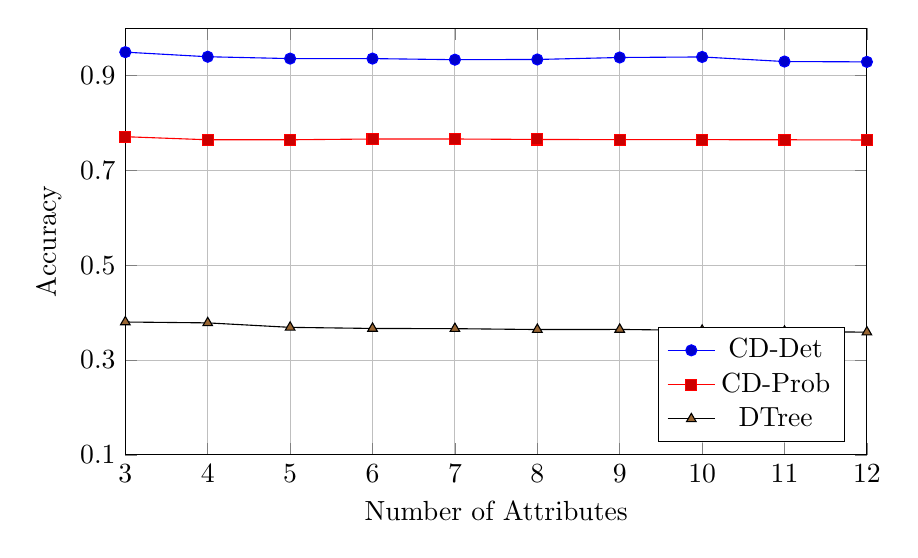
\begin{tikzpicture}
        \begin{axis}[
            width=11cm,
            height=7cm,
            xlabel={Number of Attributes},
            ylabel={Accuracy},
            xmin=3, xmax=12,
            ymin=0.1, ymax=1.0,
            xtick={3,4,5,6,7,8,9,10,11,12},
            ytick={0.1,0.3,0.5,0.7,0.9},
            legend pos=south east,
            grid=major,
            mark options={solid}
        ]

            \addplot+[mark=*, blue] coordinates {
                (3, 0.949528) (4, 0.939848) (5, 0.93593) (6, 0.93593) (7, 0.933625) (8, 0.934086) (9, 0.938235) (10, 0.939387) (11, 0.929707) (12, 0.929016)
            };
            \addlegendentry{CD-Det}

            \addplot+[mark=square*, red] coordinates {
                (3, 0.771145) (4, 0.764692) (5, 0.764692) (6, 0.766306) (7, 0.766306) (8, 0.765384) (9, 0.764923) (10, 0.764923) (11, 0.764692) (12, 0.764231)
            };
            \addlegendentry{CD-Prob}

            \addplot+[mark=triangle*, black] coordinates {
                (3, 0.380272) (4, 0.378428) (5, 0.368979) (6, 0.366674) (7, 0.366213) (8, 0.36437) (9, 0.3646) (10, 0.362526) (11, 0.360452) (12, 0.358838)   };
            \addlegendentry{DTree}

        \end{axis}
    \end{tikzpicture}\label{fig:f2-results}
\end{figure}

The results, shown in Figures~\ref{fig:f1-results} and~\ref{fig:f2-results}, reveal notable differences in
performance depending on the underlying class assignment rule.
For function $f_1$, both deterministic and probabilistic methods achieve high accuracy, with the deterministic
version of the central distribution slightly outperforming the other.
In contrast, function $f_2$ introduces more ambiguity in the label assignment, leading to a clearer separation
in performance between these two methods.
In this case, the deterministic central distribution remains the most accurate overall, while the probabilistic
version shows reduced performance due to label overlap.


\begin{figure}[htbp]
    \centering
    \caption{Accuracy vs. Number of Attributes (Function $f_2$, 10 train samples)}
    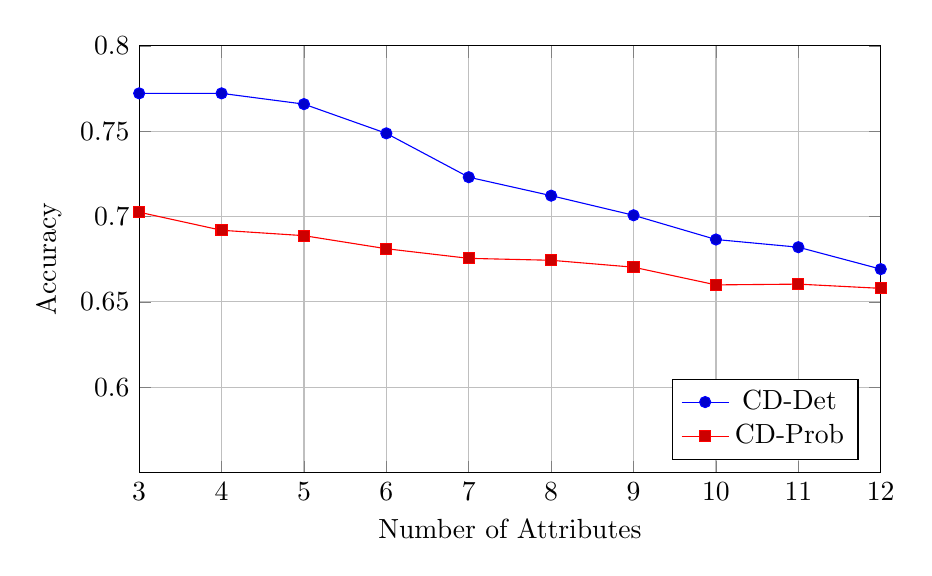
\begin{tikzpicture}
        \begin{axis}[
            width=11cm,
            height=7cm,
            xlabel={Number of Attributes},
            ylabel={Accuracy},
            xmin=3, xmax=12,
            ymin=0.55, ymax=0.8,
            xtick={3,4,5,6,7,8,9,10,11,12},
            ytick={0.6,0.65,0.7,0.75,0.8},
            legend pos=south east,
            grid=major,
            mark options={solid}
        ]

            \addplot+[mark=*, blue] coordinates {
                (3, 0.772143) (4, 0.772143) (5, 0.765833) (6, 0.748704) (7, 0.723011) (8, 0.712193) (9, 0.700699) (10, 0.6865) (11, 0.681992) (12, 0.669146)
            };
            \addlegendentry{CD-Det}

            \addplot+[mark=square*, red] coordinates {
                (3, 0.702502) (4, 0.691909) (5, 0.688754) (6, 0.681091) (7, 0.675456) (8, 0.67433) (9, 0.670273) (10, 0.659905) (11, 0.660356) (12, 0.657877)
            };
            \addlegendentry{CD-Prob}

        \end{axis}
    \end{tikzpicture}\label{fig:f2-10samples-results}
\end{figure}

While removing irrelevant attributes generally led to slight improvements in accuracy, the effect was not
substantial in our primary experiments with 20 training samples.
However, we observed that the benefit of attribute removal becomes more noticeable when the training set is
smaller.
In particular, additional experiments with only 10 training samples showed a clearer performance gain as
irrelevant features were removed, indicating that the impact of irrelevant attributes is more pronounced in
low-data regimes (see Figure~\ref{fig:f2-10samples-results})
